%%%%%%%%%%%%%%%%%%%%%%%%%%%%%%%%%%%%%%%%%%%%%%%%%%%%%%%%%%%%%%%%%%%%%%%%%%%%
% AGUJournalTemplate.tex: this template file is for articles formatted with LaTeX
%
% This file includes commands and instructions
% given in the order necessary to produce a final output that will
% satisfy AGU requirements, including customized APA reference formatting.
%
% You may copy this file and give it your
% article name, and enter your text.
%
% guidelines and troubleshooting are here: 

%% To submit your paper:
\documentclass[draft]{agujournal2019} % 
\usepackage{url} %this package should fix any errors with URLs in refs.
\usepackage{lineno}
\usepackage[inline]{trackchanges} %for better track changes. finalnew option will compile document with changes incorporated.
\usepackage{soul}
%\linenumbers

% j'ai rajouté ce qui suit ----
\newcommand{\FC}[1]{{\color{purple}{{Fleur: ~#1}}}}
\newcommand{\Fc}[1]{{\color{purple}{{Fleur: ~#1}}}}
\newcommand{\AL}[1]{{\color{orange}{{Alex: ~#1}}}}
\newcommand{\Al}[1]{{\color{orange}{{Alex: ~#1}}}}
\newcommand{\HJ}[1]{{\color{blue}{{Hugo: ~#1}}}}
\usepackage{amsmath}
%\usepackage{subcaption,tikz,makecell}
%\DeclareRobustCommand\sampleline[1]{%
%	\tikz\draw[#1] (0,0) (0,\the\dimexpr\fontdimen22\textfont2\relax)
%	-- (2em,\the\dimexpr\fontdimen22\textfont2\relax);%
%} % see https://tex.stackexchange.com/questions/280726/how-to-show-line-symbol-in-text

%TC:macro \cite [option:text,text]
%TC:macro \citeA [option:text,text]
\usepackage{verbatim}
\newcommand{\detailtexcount}[1]{%
  \immediate\write18{texcount -merge -sum -q #1.tex output.bbl > #1.wcdetail }%
  \verbatiminput{#1.wcdetail}%
}
\newcommand{\quickwordcount}[1]{%
  \immediate\write18{texcount -1 -sum -merge -q #1.tex output.bbl > #1-words.sum }%
  \input{#1-words.sum} words%
}
\newcommand{\quickcharcount}[1]{%
  \immediate\write18{texcount -1 -sum -merge -char -q #1.tex output.bbl > #1-chars.sum }%
  \input{#1-chars.sum} characters (not including spaces)%
}

% -----------------------------


%%%%%%%
% As of 2018 we recommend use of the TrackChanges package to mark revisions.
% The trackchanges package adds five new LaTeX commands:
%
%  \note[editor]{The note}
%  \annote[editor]{Text to annotate}{The note}
%  \add[editor]{Text to add}
%  \remove[editor]{Text to remove}
%  \change[editor]{Text to remove}{Text to add}
%
% complete documentation is here: http://trackchanges.sourceforge.net/
%%%%%%%

\draftfalse % \drafttrue draftfalse


%% Enter journal name below.
%% Choose from this list of Journals:
%
% JGR: Atmospheres
% JGR: Biogeosciences
% JGR: Earth Surface
% JGR: Oceans
% JGR: Planets
% JGR: Solid Earth
% JGR: Space Physics
% Global Biogeochemical Cycles
% Geophysical Research Letters
% Paleoceanography and Paleoclimatology
% Radio Science
% Reviews of Geophysics
% Tectonics
% Space Weather
% Water Resources Research
% Geochemistry, Geophysics, Geosystems
% Journal of Advances in Modeling Earth Systems (JAMES)
% Earth's Future
% Earth and Space Science
% Geohealth
%
% ie, \journalname{Water Resources Research}

\journalname{JGR: Atmospheres}


\begin{document}

    
	%%%%%%%%%%%%%%%%%%%%%%%%%%%%%%%%%%%%%%%%%%%%%%%
	%  TITLE
	%
	% (A title should be specific, informative, and brief. Use
	% abbreviations only if they are defined in the abstract. Titles that
	% start with general keywords then specific terms are optimized in
	% searches)
	%
	%%%%%%%%%%%%%%%%%%%%%%%%%%%%%%%%%%%%%%%%%%%%%%%
	
	% Example: \title{This is a test title}
	
	\title{Linking surface roughness with vertical coherent structures in the marine boundary layer near the Agulhas current}
	
	% avec une note structure coherente :
    %   Atmosphere Response To An Oceanic Sub-mesoscale SST Front: A Coherent Structure Analysis
	% le classique : Atmosphere Response To An Oceanic Sub-mesoscale SST Front
 
	%%%%%%%%%%%%%%%%%%%%%%%%%%%%%%%%%%%%%%%%%%%%%%%
	%
	%  AUTHORS AND AFFILIATIONS
	%
	%%%%%%%%%%%%%%%%%%%%%%%%%%%%%%%%%%%%%%%%%%%%%%%
	
	% Authors are individuals who have significantly contributed to the
	% research and preparation of the article. Group authors are allowed, if
	% each author in the group is separately identified in an appendix.)
	
	% List authors by first name or initial followed by last name and
	% separated by commas. Use \affil{} to number affiliations, and
	% \thanks{} for author notes.
	% Additional author notes should be indicated with \thanks{} (for
	% example, for current addresses).
	
	% Example: \authors{A. B. Author\affil{1}\thanks{Current address, Antartica}, B. C. Author\affil{2,3}, and D. E.
		% Author\affil{3,4}\thanks{Also funded by Monsanto.
			
			\authors{Hugo Jacquet\affil{1}, Alex Ayet\affil{2}, Fleur Couvreux\affil{3}}
			
			\affiliation{1}{Université Grenoble Alpes, CNRS, IGE, France}
			\affiliation{2}{CNRS, Université Grenoble Alpes, Inria, Grenoble INP,  GIPSA-Lab, Grenoble, France.}
			\affiliation{3}{Université de Toulouse, Météo-France, CNRS, CNRM, France}
			
			\correspondingauthor{Hugo Jacquet}{hugo.jacquet.work@gmail.com}
			
			
			
			%%%%%%%%%%%%%%%%%%%%%%%%%%%%%%%%%%%%%%%%%%%%%%%
			% KEY POINTS
			%%%%%%%%%%%%%%%%%%%%%%%%%%%%%%%%%%%%%%%%%%%%%%%
			%  List up to three key points (at least one is required)
			%  Key Points summarize the main points and conclusions of the article
			%  Each must be 140 characters or fewer with no special characters or punctuation and must be complete sentences
			
			% Example:
			% \begin{keypoints}
				% \item	List up to three key points (at least one is required)
				% \item	Key Points summarize the main points and conclusions of the article
				% \item	Each must be 140 characters or fewer with no special characters or punctuation and must be complete sentences
				% \end{keypoints}
			
			%\begin{keypoints}
			%\item enter point 1 here
			%\item enter point 2 here
			%\item enter point 3 here
			%\end{keypoints}
			
			%%%%%%%%%%%%%%%%%%%%%%%%%%%%%%%%%%%%%%%%%%%%%%%
			%
			%  ABSTRACT and PLAIN LANGUAGE SUMMARY
			%
			% A good Abstract will begin with a short description of the problem
			% being addressed, briefly describe the new data or analyses, then
			% briefly states the main conclusion(s) and how they are supported and
			% uncertainties.
			
			% The Plain Language Summary should be written for a broad audience,
			% including journalists and the science-interested public, that will not have 
			% a background in your field.
			%
			% A Plain Language Summary is required in GRL, JGR: Planets, JGR: Biogeosciences,
			% JGR: Oceans, G-Cubed, Reviews of Geophysics, and JAMES.
			% see http://sharingscience.agu.org/creating-plain-language-summary/)
			%
			%%%%%%%%%%%%%%%%%%%%%%%%%%%%%%%%%%%%%%%%%%%%%%%
			
			%% \begin{abstract} starts the second page
				
				\begin{abstract}
                   
				\end{abstract}
                To be done



    
				\section*{Plain Language Summary}
				To be done
				%Here are instructions on writing a Plain Language Summary: 
				%https://www.agu.org/Share-and-Advocate/Share/Community/Plain-language-summary
				
				
				%%%%%%%%%%%%%%%%%%%%%%%%%%%%%%%%%%%%%%%%%%%%%%%
				%
				%  BODY TEXT
				%
				%%%%%%%%%%%%%%%%%%%%%%%%%%%%%%%%%%%%%%%%%%%%%%%
				
				
				% checklist here : https://www.agu.org/publications/authors/journals/submission-checklists
                % In-Depth Text and Graphics Requirements : https://www.agu.org/publications/authors/journals/text-graphics-requirements
                % Grammar : https://www.agu.org/publish-with-agu/publish/author-resources/grammar-style-guide
				
				
        \section{Introduction}
        \label{section_introduction}
        
        % General need
        Vocabulary:\\
        MABL = Marine Atmospheric Boundary Layer \\
        Coherent structure = object detected by \cite{couvreux_resolved_2010} that maximize the contribution of objects to the turbulent fluxes ($<$uw$>$ and $<$w$\theta_v$$>$)\\

        Work hypothesis :
        \begin{itemize}
            \item Coherent structure of the MABL can be seen on SAR surface data.
            \item Coherent structure of the MABL can be detected with a conditionial sampling based on passive tracer emission.
        \end{itemize}

        % Specific need that we will adress / Scientific question
        The main goal of this study is to answer the following questions:
        \begin{itemize}
            \item What is the internal structure of the MABL above a realistic SST front and how is it influenced by environmental conditions ?
            \item Can surface roughness retrieved from SAR satellite give information about the vertical structure of the MABL ?
        \end{itemize}
        
        % Tools to answer a scientific question
        % - LES
        % - Conditional sampling
        % - High res images of SAR

        % Plan
        
        \section{The LES simulations} 
        \label{subsection_numerical_setup}     
        
            % Petit paragraphe pour décrire le model (faire ref à canal_sim)
            % Petit para. pour décrire la difficulté à faire des LES au dessus d'hétérogénéités

            

            \subsection{General considerations}
            \label{subsection_general_principle}
            
            Modeling a flow over an heterogeneity is a challenge \cite{fogarty_how_2024}. To address this, we design the experiment illustrated on Figure \ref{nesting_setup}. We use the nesting capabilities of MesoNH \cite[version 5.7.0]{lac_overview_2018} : two simulations are run in the same experiment. A first domain with low resolution is set up and we will call this domain the `dad' domain. Lateral boundary conditions are cyclic in the West/East direction, and open in the North/South direction. This domain serves as a turbulence generator that will be injected in the second domain (the `son' domain). The exchange of information is one way, meaning that the son is influenced by the dad but not the other way. The hope in such design is that the inflow characteristics will be improved compared to a son-only equivalent simulation with double open boundary conditions and with a shorter distance for the turbulence to develop. The validation of the inflow will be detailed in the section \ref{subsection_inflowvalid}. Another way to have a turbulent inflow is the `turbulence recycling' method described by \citeA{nagel_numerical_2022} but it has only been tested in neutral conditions and we focus here on a heterogeneous SST gradient (in both X and Y directions) and so this second method would have required more testing before use.

            \begin{figure}[h]
				\centering
				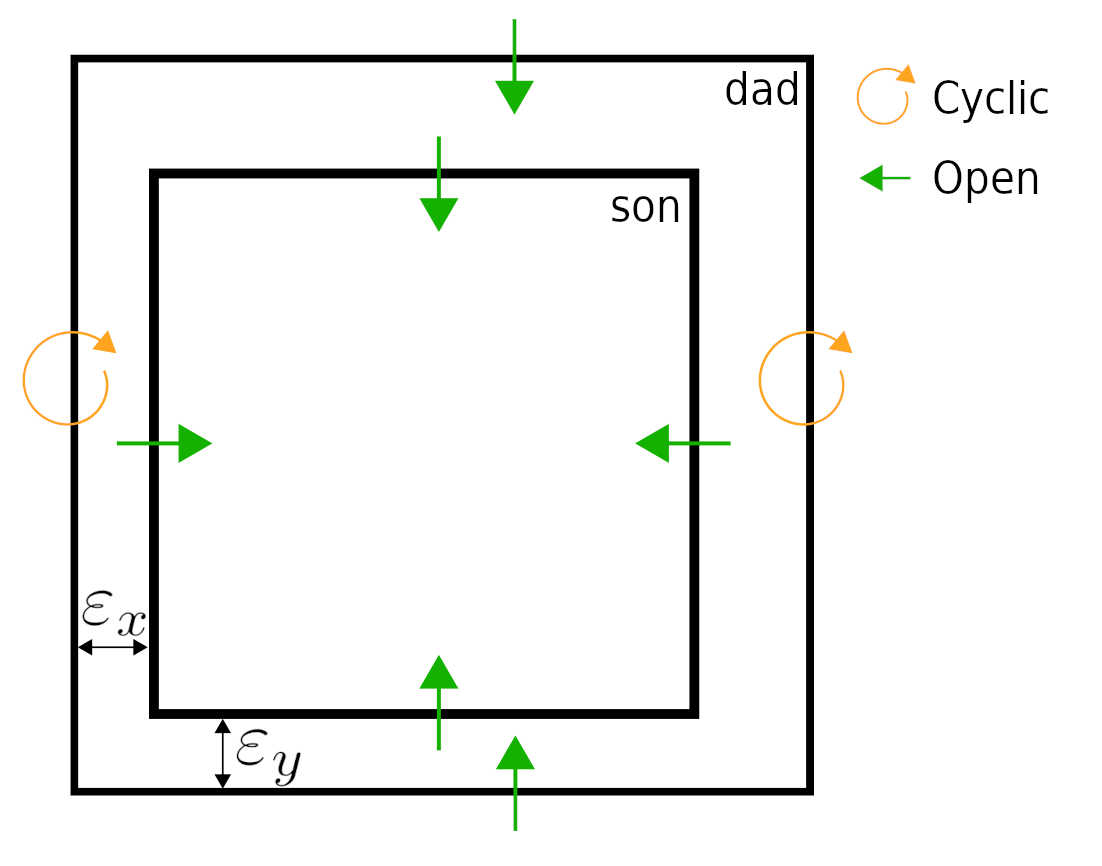
\includegraphics[width=0.5\textwidth]{Nesting_setup_modified.png}
				\caption{Nesting configuration. Arrows are the boundary conditions for each domains.}
				\label{nesting_setup}
			\end{figure}
            % rajouter 'X' et 'Y' ou des axes

            We now describe the general configurations of the simulations. Two set of simulations have been produced: a turbulent inflow validation set (described in Section \ref{subsection_inflowvalid}) and an experiment with a realistic SST. All simulations use the same physic, meaning they have the same cloud scheme and subgrid turbulence parametrizations and they also use the same discretization (CEN4TH,RK4,PPM01) of the equations of conservation. The numerical schemes and parametrizations used here are the same as in \citeA{jacquet_atmosphere_2025}. All simulations use the same vertical levels, ranging from $\Delta_z$ = 2 m at the surface to $\Delta$z = 20 m at Z = 2000 m, the model top. Horizontal grid spacing is uniform and it is the same in X and Y directions. The horizontal resolution $\Delta_{x}$ is 200 m for the dad domains, and 50 m for son domains as well as any homogeneous cyclic configurations. Characteristics specific to each simulations can been found in the Table \ref{tab:setups}. When using the fourth order central finite difference scheme and fourth order Runge-Kutta for spatial and temporal discretizations for wind advection, a diffusion operator is applied on wind variables to reduce spurious motions. This characteristic time is XT4DIFU and it has to be tuned by the user according to the resolution of the experiment. In our case, a usual value of XT4DIFU = 100 s is used for domains at 50 m resolution, which damp 2$\Delta_x$ waves by $e^{-1}$ in 10 timesteps. A value of XT4DIFU = 800 s for the domains at 200 m was found to improve the turbulent inflow for the son domains, compared to a dad domain with a stronger diffusion. The son domain is defined after a period of spinup from the dad domain. The spinup time is one hour for the validation experiment and \textbf{???} for the experiment with the realistic SST. Then, the grid of the son domain is defined by $\varepsilon_x$ and $\varepsilon_y$ which are the number of cells way from the eastern and southern boundaries respectively (in number of cell from the dad domain). We choose to set $\varepsilon_y$ in a way that put the the son domain as far as possible to the open boundary condition from the dad domain.  $\varepsilon_x$ is set to be close the the boundary as the dad East boundary condition is cyclic and thus we do not expect any problem with this type of boundary. 

            % a discuter ? XT4DIFU=1800s pour le père permet d'avoir un inflow plus propre pour le fils.

            \begin{table}[h]
                \caption{Configuration of the simulations}
				\centering
				\begin{tabular}{ccccccccc}
					\hline
                    Name & $\Delta_{x}$ (m) & $\Delta_t$ (s) & XT4DIFU (s) & $N_x$ & $N_y$ & $\varepsilon_x$ & $\varepsilon_y$ & SST\\
                    \hline
                    \textbf{Validation} \\
					VALdad & 200   & 4 & 800 & 64 & 64 & 0 & 0 & N/S gradient or 298 K\\
					VALson & 50    & 1 & 100  & 200 & 200 & 4 & 4 & N/S gradient or 298 K\\
                    RefVal & 50    & 1 & 100  & 200 & 200 & 4 & 4 & 298 K\\
                    \textbf{Experiment} \\
                    AGGdad & 200   & 4 & 800 & TBD & TBD & 0 & 0 & analysis\\
					AGGson & 50    & 1 & 100  & TBD & TBD & TBD & TBD & analysis\\
                    RefC & 50 & 1 & 100  & 200 & 200 & - & - & TBD\\
                    RefW & 50 & 1 & 100  & 200 & 200 & - & - & TBD\\
					\hline
				\end{tabular}
				\label{tab:setups}
			\end{table}

            
            
            \subsection{Turbulent inflow validation}
            \label{subsection_inflowvalid}

            % discter condition ouverte N/S pour le père -> car gradient SST N/S
            This section aims to validate the nesting configuration of Figure \ref{nesting_setup} as a way to get a turbulent inflow for a LES simulation over an heterogeneity. At first, a nested setup is designed with homogeneous SST of 298 K, giving a fairly convective atmosphere ($z_i/L$ = ?). The characteristics of the dad (VALdad) and son (VALson) domains can be found in Table \ref{tab:setups}. For comparison, a simulation with homogeneous SST (298 K) and cyclic conditions has been run (RefVal in Table \ref{tab:setups}). Initial conditions are the same for the two simulations: a constant, zonal-only geostrophic wind of 7.5 $m.s^{-1}$, an idealized boundary layer with constant potential temperature $\theta$ = 295 K and moisture mixing ratio $r_v$ = 10 $g.kg^{-1}$ under $z_i$ and then a gradient of temperature (3 K.km$^{-1}$) and moisture  (-4,6 g.kg$^{-1}$.km$^{-1}$). After two hours of simulated time, Figure \ref{VAL_homo_WT_200m} shows vertical wind. The homogeneous simulation show convective plumes of ? the size of the domain. The son domain from the nested configuration has a smooth turbulent inflow coming at turbulent scale of the dad domain. The fetch needed for the turbulence to become `at scale' (in the sens of \citeA{nagel_numerical_2022}) can be qualitatively seen by spotting the distance where the turbulent structure are not as smooth as the inflow. In this case, we estimate the fetch at around 6 km away from the inflow border, in the zonal direction. We note however that structures from the VALson simulation cover more area than the RefVal case. To validate the fetch quantitatively, we show on Figure \ref{VAL_homo_spectra_several_X} cross-wind spectra at several X position (the dominant wind is zonal) and we compare them with the spectrum at the East border of VALson and also cross-wind spectra from RefVal. Spectra show that i) turbulence near the East border of VALson is comparable to the spectra from the homogeneous simulation, meaning that the turbulent scales are now similar to a non-nested configuration ii) the turbulent fecth from the West border of VALson is around 4 km, 2 km earlier from the qualitative value. The second point means that the fetch can be first detected `by eye' during a design phase of the setup, and then confirmed with spectra later. This fetch is far less than what was found in a similar configuration but with an open inflow boundary condition that required more than 20 km for turbulence to develop from the inflow condition (a prescribed profile with no perturbation).     
            % voir X500_warmer
            
            \begin{figure}[h]
				\centering
				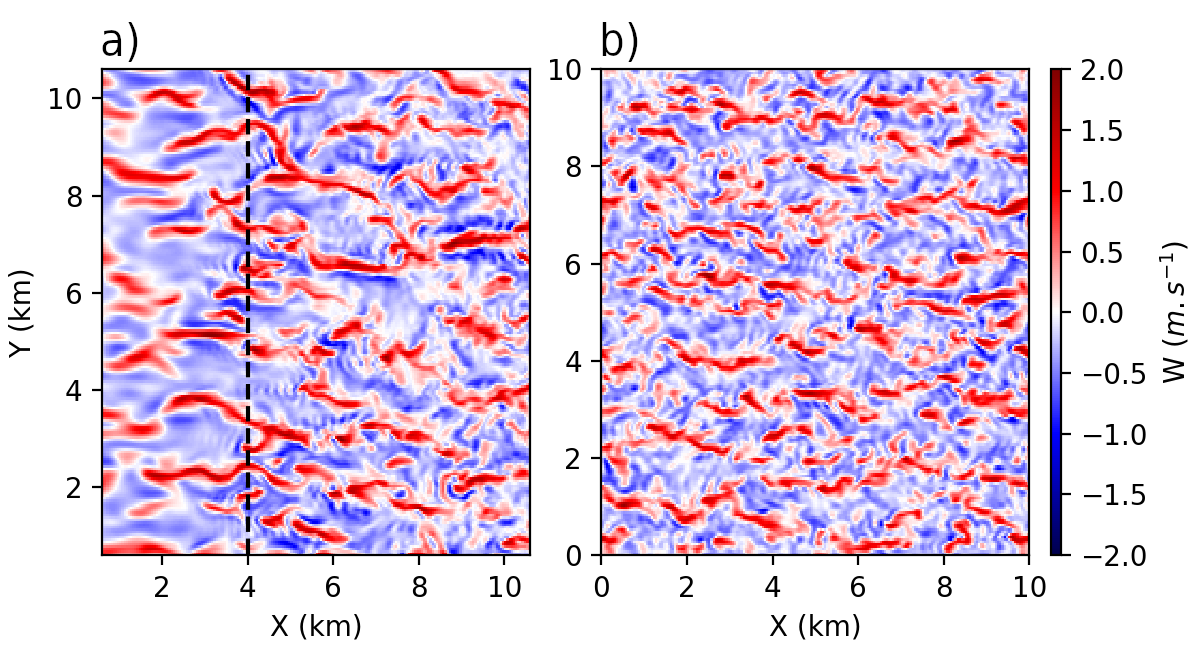
\includegraphics[width=0.85\textwidth]{Overview_W_atZ200m_nest_homo_c.png}
				\caption{Vertical velocity at Z = 200 m for the simulations a) VALson with homogeneous SST and b) RefVal. The vertical dashed line on a) discriminate turbulent scale from dad (left of the line) and son (right of the line) domains.}
				\label{VAL_homo_WT_200m}
			\end{figure}
   
            \begin{figure}[h]
				\centering
				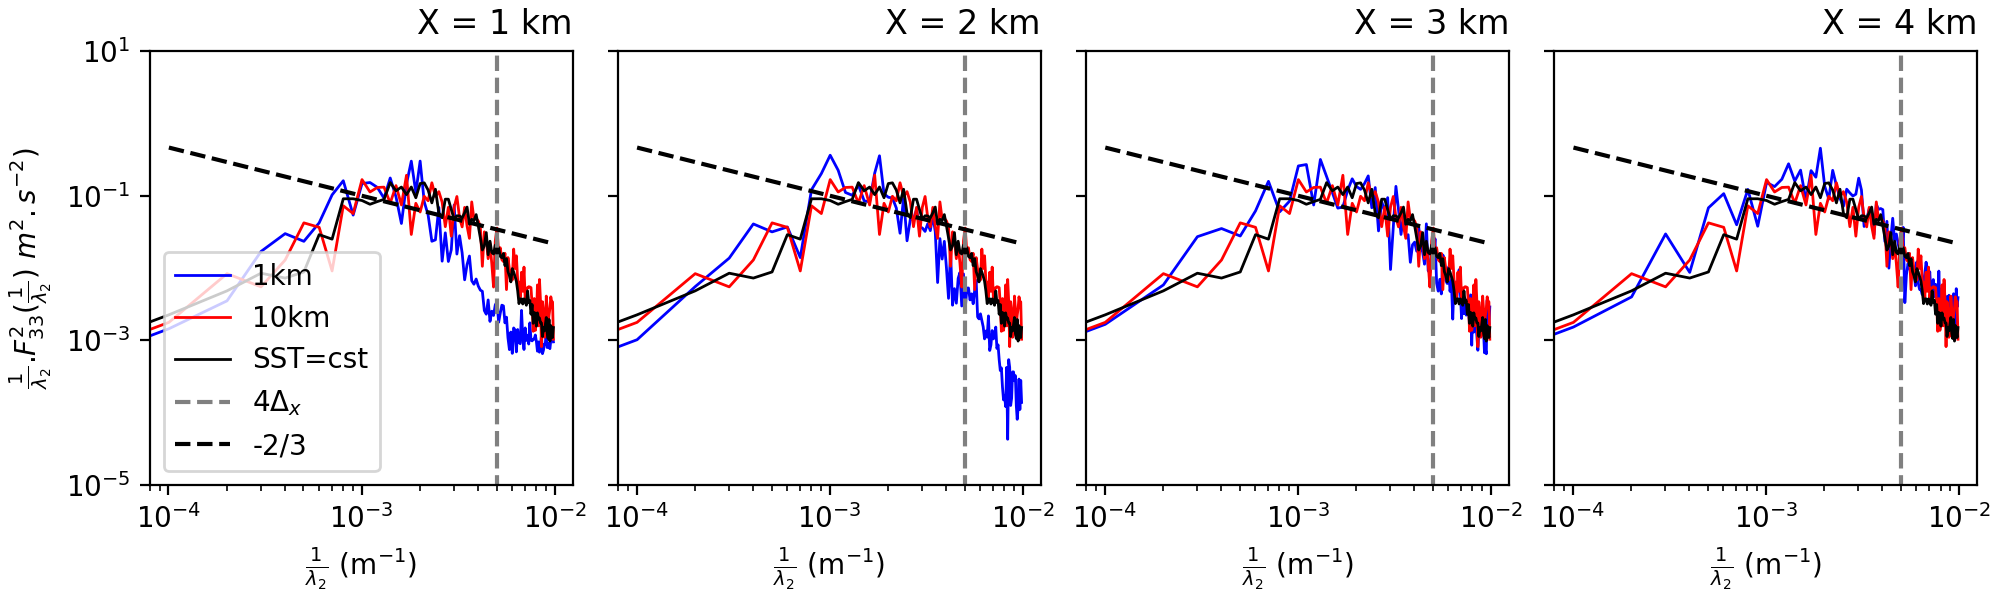
\includegraphics[width=0.99\textwidth]{KPSD_W_atZ200_X1234vs10km.png}
				\caption{Cross-wind spectra of vertical velocity at Z = 200 m, at several X position (in blue) for VALson, at X = 10 km (West side of the domain, in red) and for the homogeneous simulation (in black). The grey vertical dashed line is the expected effective resolution of 4$\Delta_x$, the black dashed line is the inertial range. Both axis are in log scale.}
				\label{VAL_homo_spectra_several_X}
			\end{figure} 
            % A la limite cette figure pas besoin, on peut juste dire que fetch ~ 5km puis fournir au reviewer la figure avec tous les spectres !
            % a faire : agrandir les xlabel ylabel
            
            Having compared turbulent scales, we now compare on Figure \ref{VAL_homo_profiles} profiles of mean quantities for VALson and RefVal. The average operator in the RefVal simulation is an horizontal average over the whole domain, while the for the VALson simulation the average is an horizontal average over the part of the domain where turbulence is `at scale', i.e. from X = 6 km to the East border. Flux are the sum of resolved and subgrid fluxes. Overall, first order statistics profiles are very similar, with a zonal velocity (Figure \ref{VAL_homo_profiles}a) from VALson slower by 5 $cm.s^{-1}$ and a better mixed moisture mixing ratio (Figure \ref{VAL_homo_profiles}c) in the nested configuration. Turbulent statistics show some discrepancy: $<uw>$ profiles from VALson might not be converged, as the average operator has around half the number of points compared to RefVal, buoyancy profiles show good agreement, total turbulent kinetic energy levels from VALson near surface (in the upper ABL) are on par with (higher than) RefVal values. 
            
            We find that the nesting configuration with homogeneous SST and the cyclic configuration gives comparable results and so we will use the nesting method to generate a turbulent inflow over a realistic SST gradient.

            NOTE Hugo 8/10/24 : pour le cas réel, j'ai utilisé XT4DIFU = 800s pour le domaine père, alors que dans mes tests j'ai utilisé la valeur de 1800s. Peut-être qu'il faudrait mettre à jour le cas test pour que ca colle avec la valeur de XT4DIFU que je vais utiliser dans la simulation réelle finale ! 

            \begin{figure}[h!]
				\centering
				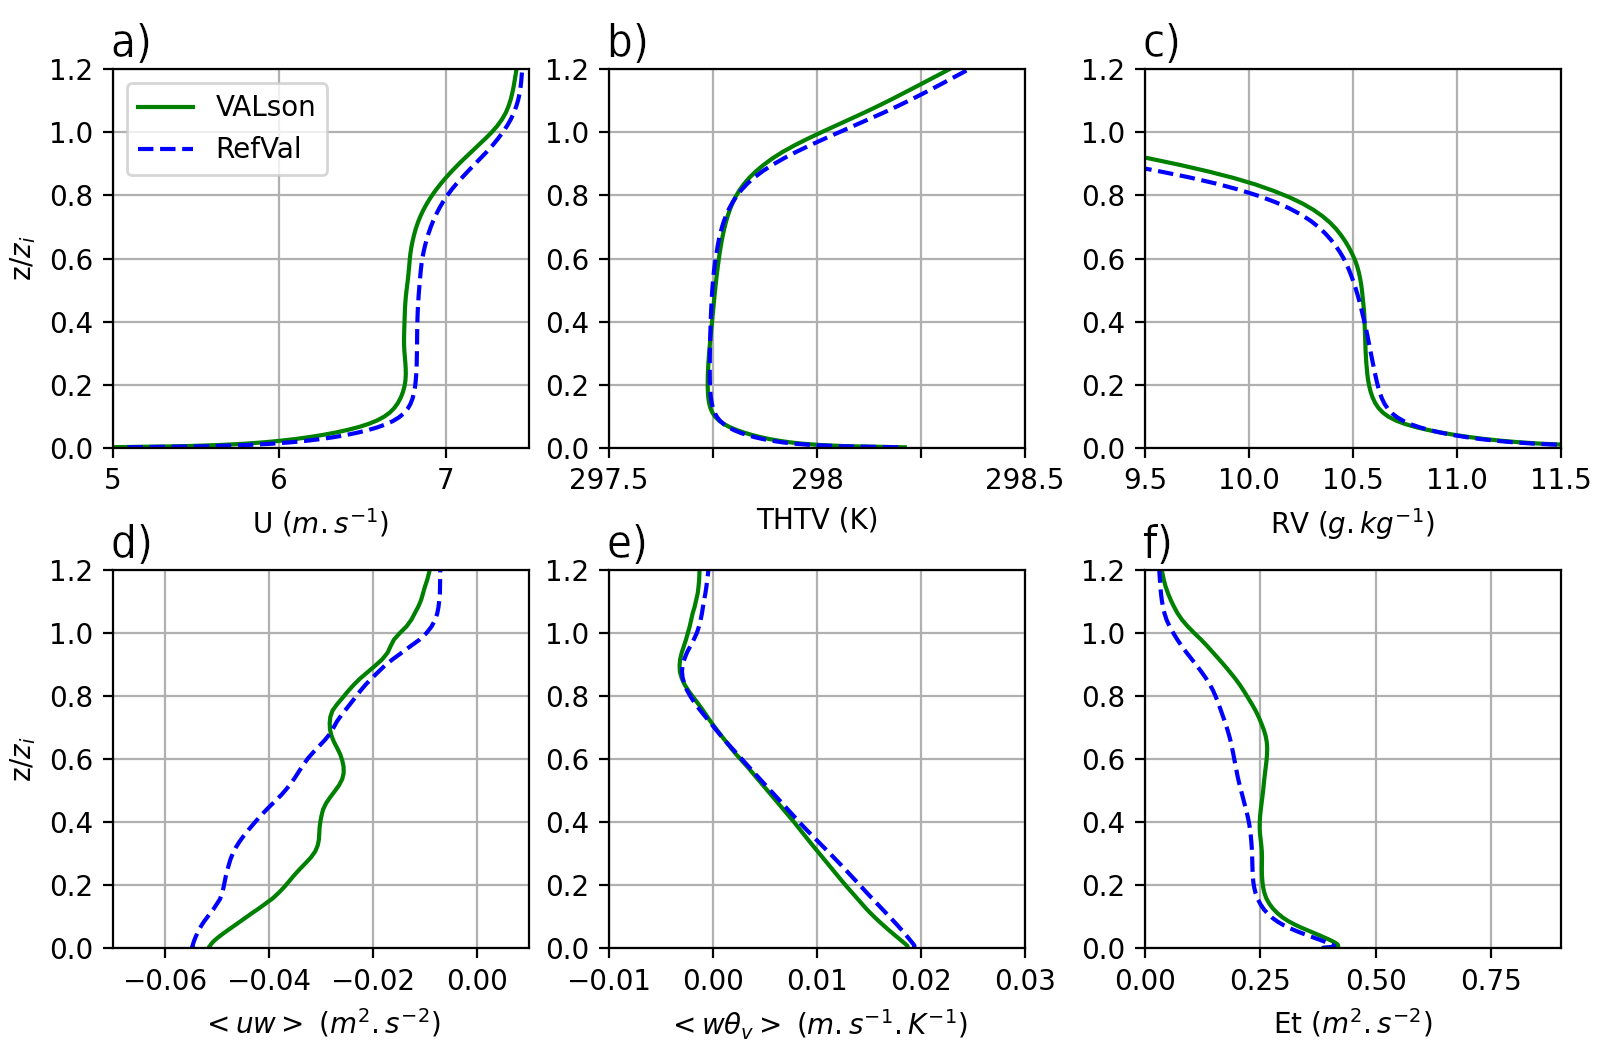
\includegraphics[width=0.99\textwidth]{Verif_combined_nestVShomo_c.png}
				\caption{Mean profiles of a) Zonal wind U ($m.s^{-1}$), b) virtual potential temperature $\theta_v$ (K), c) moisture mixing ratio $r_v$ ($g.kg^{-1}$) d) total vertical flux of zonal momentum $<$$uw$$>$ ($m^2.s^{-2}$), e) buoyancy flux $<$$w\theta_v$$>$ ($m.s^{-1}.K^{-1}$) and f) total turbulent kinetic energy Et ($m^2.s^{-2}$). See the text for the definition of the average operators.}
				\label{VAL_homo_profiles}
			\end{figure} 
            % Enlever les unité de dessous les graphs car déjà dans la légende, ca surcharge moins
            % Changer THTV pour la lettre grec

        \section{The Aghulas current}
        \label{section_overview10dec2015}
            
            % description du cas d'étude
            % - une image du visible
            % - discussion nuages/aérosols
            % - description simu LES du cas réel (principalement description SST)

            We now focus on describing the case study of the `Experiment' simulations (Table \ref{tab:setups}). A brief description of the environmental conditions is given, including an overview of the ERA5 dataset profiles.

            Here description of visible, SST L4 reanalysis, SAR vignette, ERA5 profiles/conditions

            Here small section about the characteristics of the LES with the realistic SST: 64*90km, dx=50m, size of dad is 108.

            \begin{figure}[h]
				\centering
				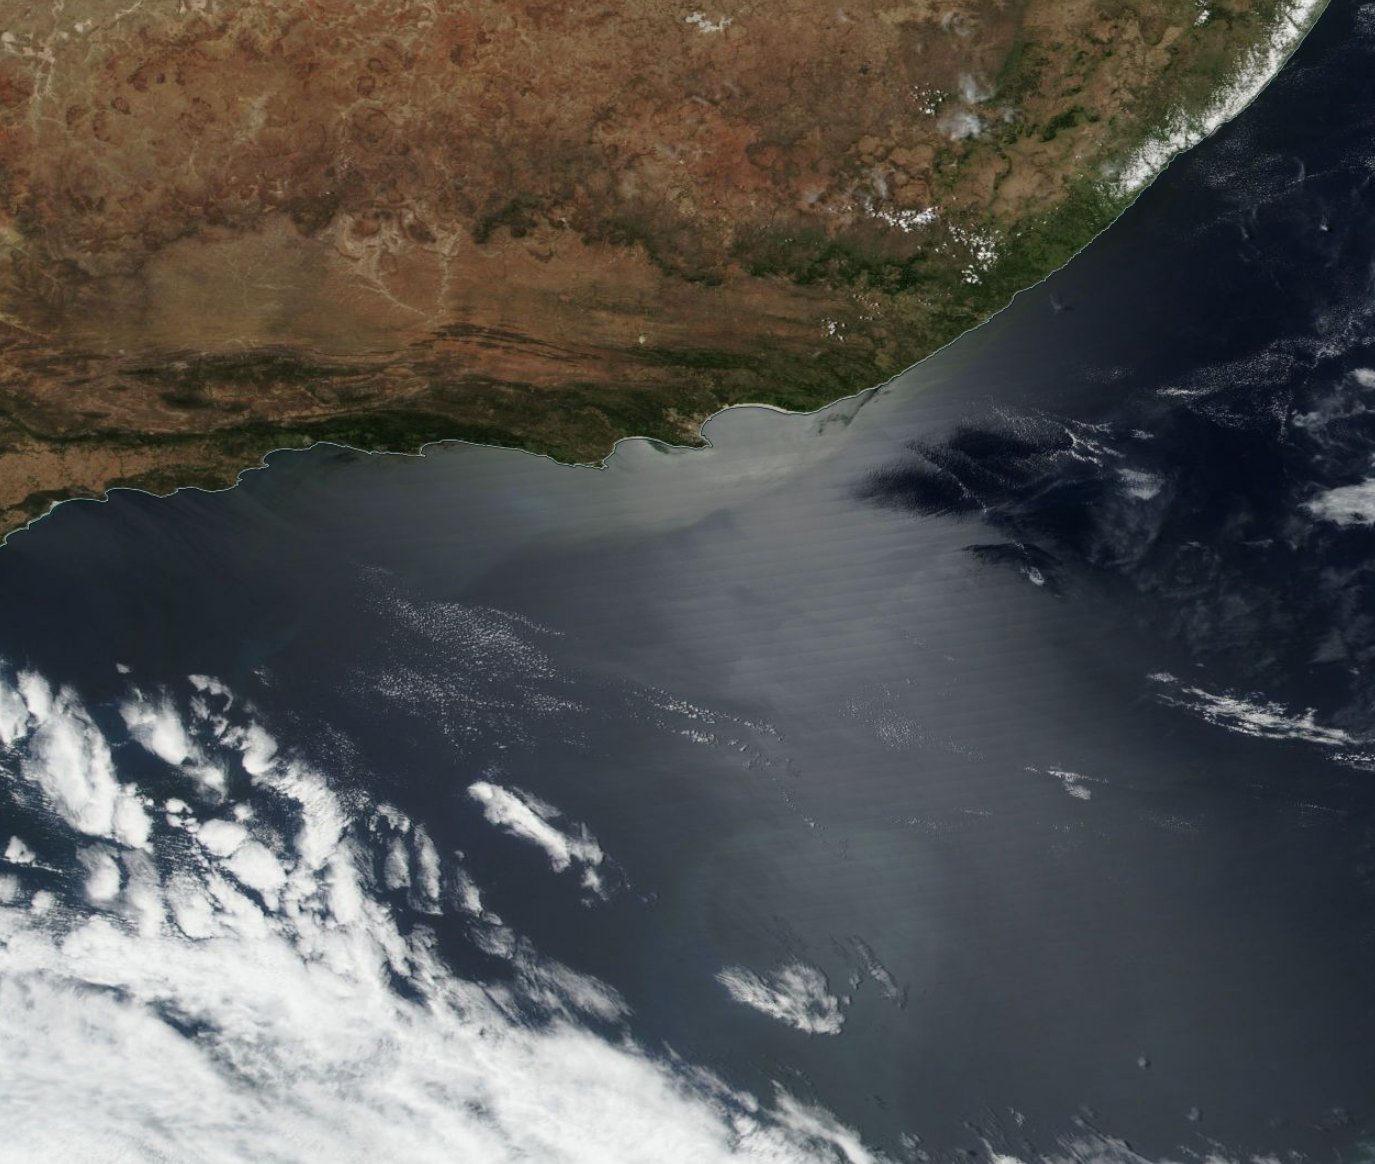
\includegraphics[width=0.6\textwidth]{aiguilles_10dec2015.png}
				\caption{Suomi NPP visible 10th dec 2015, aerosols are present. Bounds are -39°N/-32°N, 20°E/30°E.}
				\label{AG_visible}
			\end{figure} 

            \begin{figure}[h]
				\centering
				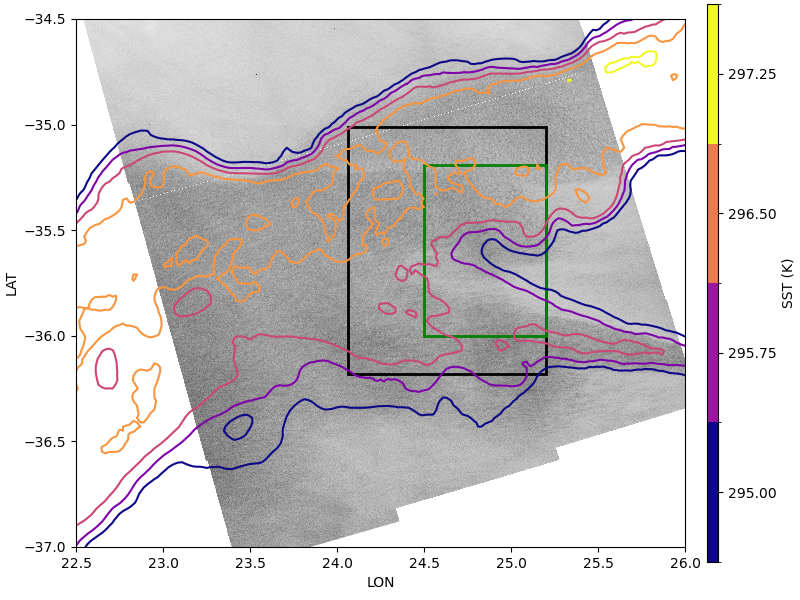
\includegraphics[width=0.6\textwidth]{SST_and_SAR.png}
				\caption{Normalized SAR roughness from Sentinel-1A, swath of the 10th of December 2015, 17h08 UTC, south of South Africa (10-12-2015 absolut orbit number 8982, numéro de vignette, product unique ID) and contours of SST from L4 Regional product from Ifremer. Rectangle are the LES domains (work in progress).}
				\label{AG_SAR_17h08UTC}
			\end{figure} 
            
        \section{Methods}
        \label{section_methods}

            For the comparison between SAR and LES images, some ideas were laid out in  \url{https://docs.google.com/document/d/1txJJcfoMKOiLx3VaDkNWp8ZrWu_z8LQwvXLLe-V5lys/edit?usp=sharing}

            \subsection{Conditional sampling based on passive tracer}
            \label{subsection_C10_description}
            Short description of the conditional sampling, link to 1rst paper

            \subsection{Spatial statistics}
            \label{subsection_SpatialStats}

                \subsubsection{Structure function}
                \label{subsubsection_structure_function}

                Structure function \cite{granero_belinchon_two-dimensional_2022} has been used to find characteristic length scale for roll organization of the ABL \cite{brilouet_trade_2023}. They are defined, in polar coordinate and at the order N, for a 2D field F, by:
                \begin{equation}
                    S_N^{r_{\theta},r_{\rho}} = < (F(r + r_{\rho}, \theta + r_{\theta} ) - F(r , \theta))^N >
                \end{equation}
                where $r$ and $\theta$ are spatial positions, $r_{\theta}$ and $r_{\rho}$ are spatial lags and $<$.$>$ is the average operator (X and Y average in our case). This structure function is computed with \textit{Nth\_structure\_function\_2D} and it uses Dask to compute in parallel $S_N^{r_{\theta},r_{\rho}}$ for each values of $r_{\theta}$ and $r_{\rho}$. On top of this, we fit an ellipse following \citeA{brilouet_trade_2023} to get characteristic length scale for the case where a roll organization is dominant. This needs to be tweaked: I still have not test case to verify that my implementation is working as intended, and also in our case there is not much roll case.

                \subsubsection{Monin-Obukhov length estimate}
                \label{subsubsection_MO_length_estimate}

                How L is estimated for SAR data \cite{odriscoll_obukhov_2023}, how we compute it in LES simulation (ref Stull).

                \subsubsection{Coherent structure characteristic size}
                \label{subsubsection_CS_characteristic_size}

                The coherent structures are detected with the C10 method. We can now look for a characteristic size of the objects. We do this by searching for an equivalent radius for each structure with the function \textit{R\_equivalent\_for\_all\_objects}. For each structure $s$ (e.g. updraft), we use \textit{scipy.ndimage.label} to label each aggregate of the structure in the plan XY. Then for each label, we take the equivalent radius as:
                \begin{equation}
                    R_{eq}(s,i,z) = ( \frac{1}{\pi} . N_i \Delta_x\Delta_y)^{1/2}
                \end{equation}
                with $N_i$ the number of cell of label $i$ at the altitude $z$ of the object $s$. We then look at the distribution of this equivalent radius at each altitude. We plot the most represented mode (in grey) and the averaged equivalent radius (in white) on Figure \ref{PDF_Requivalent_boxe2}. The mean equivalent radius is also plotted on Figure \ref{mean_req} for comparison between objects. 
                            
            \subsection{Environment influence}
            \label{subsection_Env_sensitivity}
            Here description of the environmental conditions that will be investigated. To be changed : geo wind speed, height of initial boundary layer, intensity of inversion, temperature/moisture of initial boundary layer (mixed layer part).

            Case 1 is ERA5, other cases needs to be defined.

            \begin{figure}[h!]
                \centering
                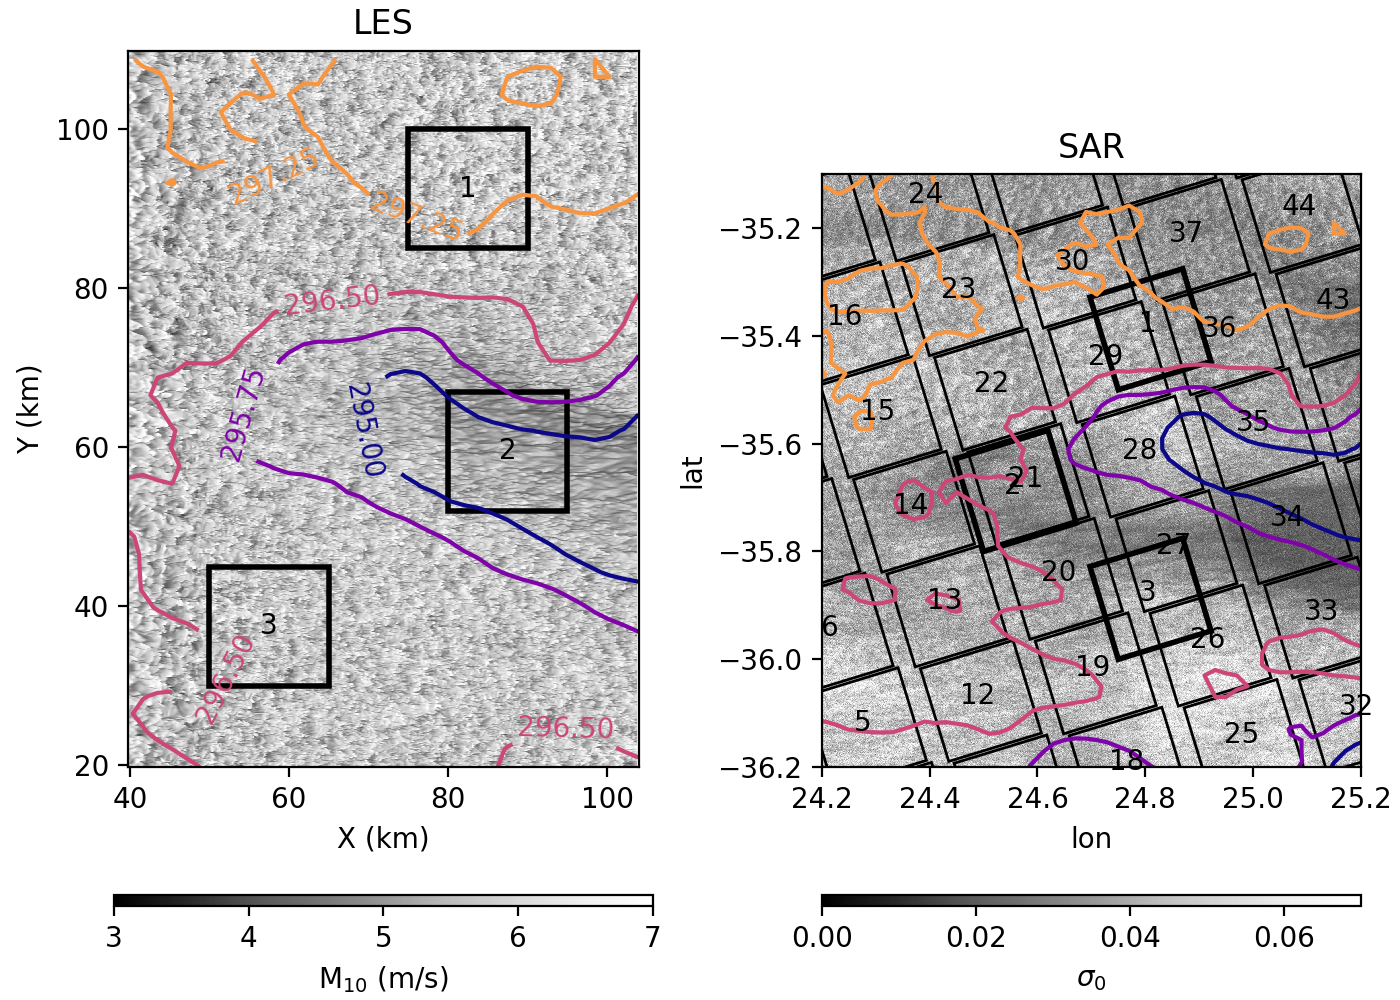
\includegraphics[width=0.99\textwidth]{Boxe_location_SAR_LES.png}
                \caption{Boxes location for SAR et LES (child domain) data. The choice of position of boxes can be automated for the SAR (it is the background of tiles numbered $>=$ 4 on the present image) but user can still specify location of interest (tiles 1 to 3 here). Background is the modulus of the 10 m wind for the LES, and the detrend surface roughness for the SAR. Contours are the SST analysis ODYSSEA.}
                \label{boxe_location}
            \end{figure} 
            
		\section{Results}
		\label{section_results}

            \subsection{Lagrangian wind budget}
            \label{subsection_wind_budget}
            % même méthode que JLR Iroise front pour calculer un budget dans une boîte qui se déplace avec le vent.

            The first step in the simulation analysis is to study the wind budget. I suggest to use a Lagrangian wind budget, much like in \citeA{redelsperger_impact_2019}. 

            \subsection{Coherent structure leaves imprints on the surface roughness}
            \label{subsection_CS_imprints_sigma0}

            Here I suggest to describe a figure with in the background a surface field (10 m wind field for example), and above this in contours the coherent structure at some altitude Z. The goal is to find visual similarities between the surface and what happens above.

            \subsection{Characteristic length scale in LES and SAR data}
            \label{subsection_scales_in_LES_and_SAR}

            Using length scale retrieved from different methods (structure functions, equivalent radius or the MO length estimate), can we find a common value for LES and SAR? And at what altitude in the LES?

            This paragraph describes Figure \ref{PDF_Requivalent_boxe2} and \ref{mean_req}. We see on Figure \ref{mean_req} that in boxe 1 and 3, the objects updraft 1 and subsiding shells 1 are not present. In all boxes, the downdrafts see a drop in $R_{eq}$ at $z_i$ or slightly above. This is because the tracer 3 is emitted the same at every altitude using a domain averaged virtual potential temperature to compute a ABL height. It is then emitted 50 m above this height. This could be improve by modifying the code to take into account local variability of $z_i$. In Figure \ref{PDF_Requivalent_boxe2}, we can see that at a specific Z and for every objects, the most represented mode (solid grey line) has a lower $R_{eq}$ than the average equivalent radius (solid white line). Typical $R_{eq}$ for up1 is greater than for up2, which is expected as boxe 2 is over a zone where only tracer 1 is emitted. Subsiding shells (ss1 and ss2) share similar values of $R_{eq}$. No downdraft are detected below the ABL height.

                \begin{figure}[h!]
    				\centering
    				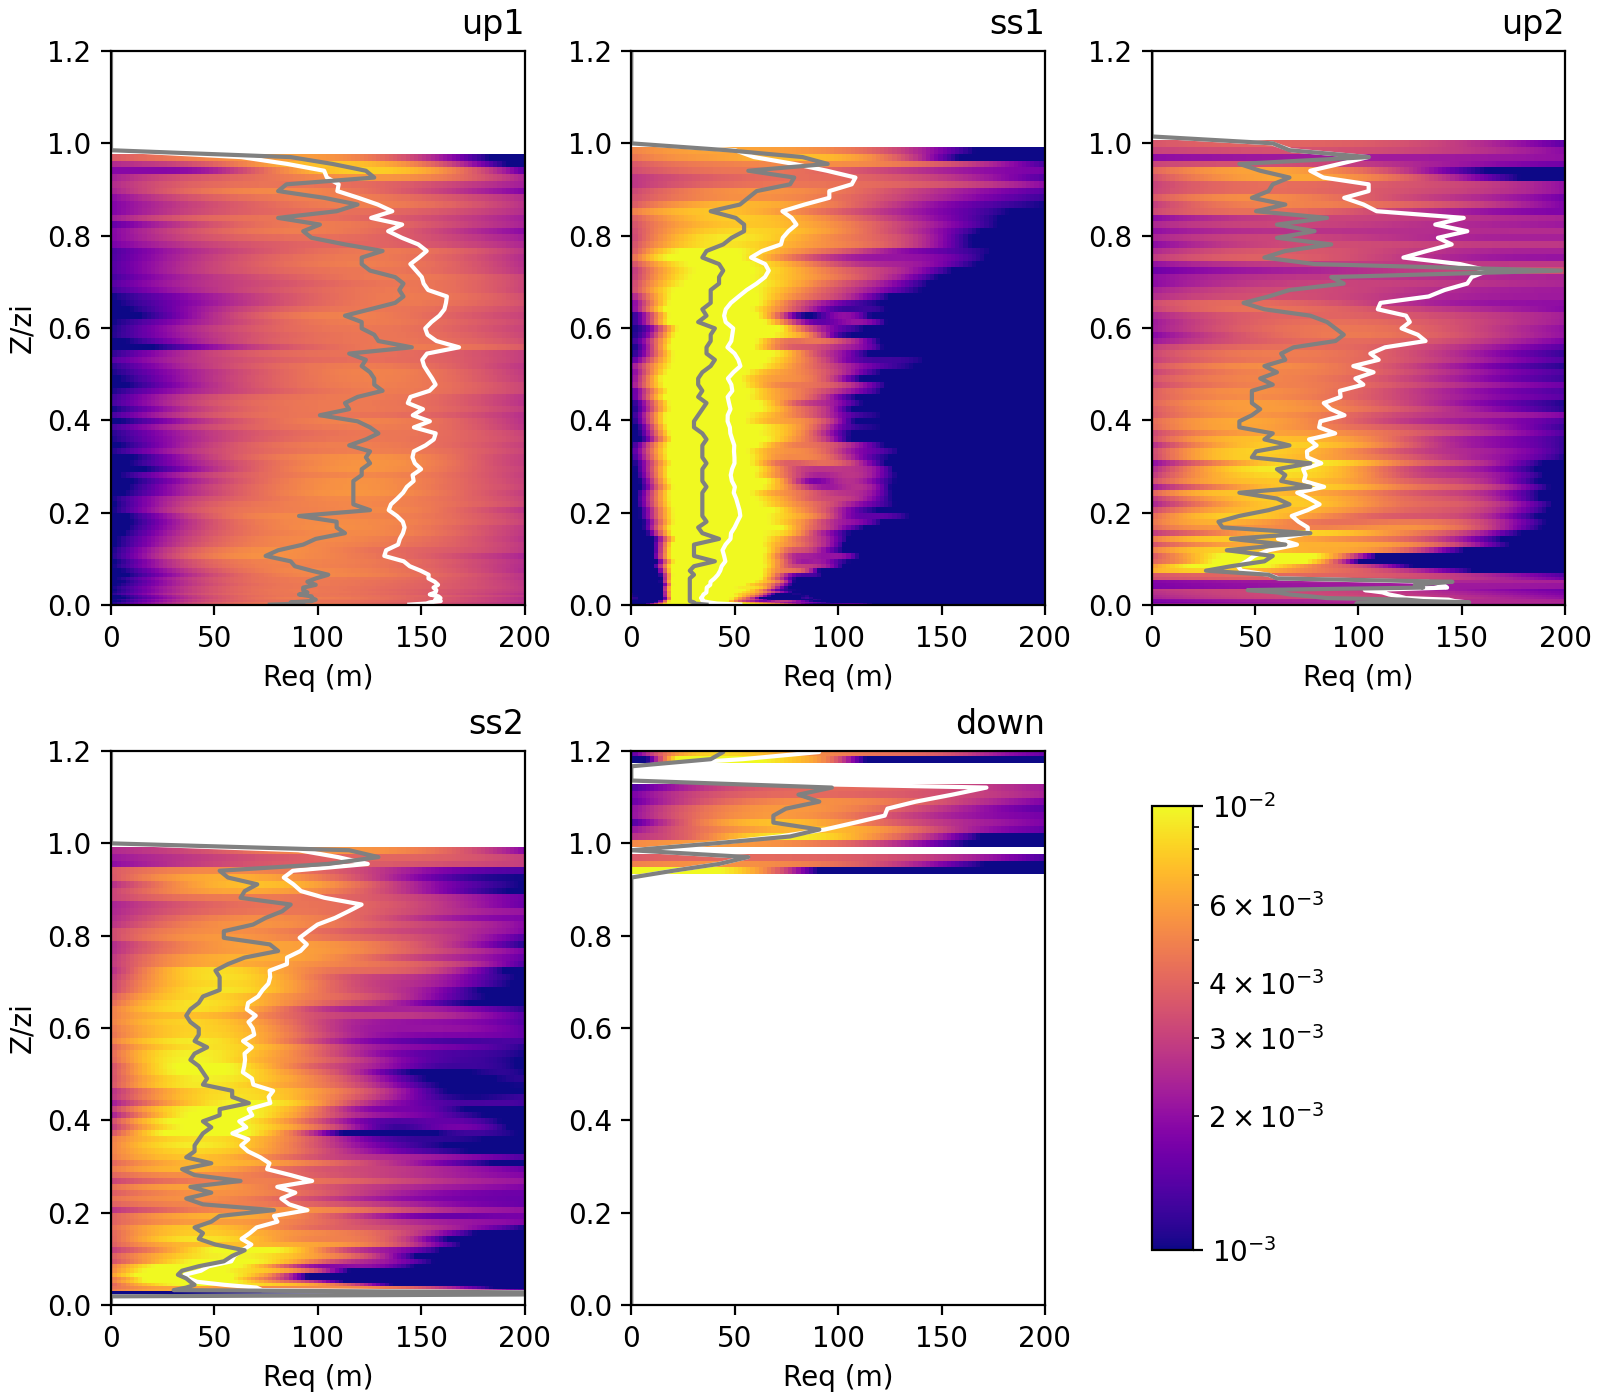
\includegraphics[width=0.99\textwidth]{PDF_Requivalent_boxe2.png}
    				\caption{LES data. PDF of equivalent radius for boxe 2 at each altitude and for each objects. Solid grey profile is the most represented mode, solid white is the averaged radius. A white background means that the object has not been detected (see Figure \ref{mean_req}).}
    				\label{PDF_Requivalent_boxe2}
			    \end{figure} 

                \begin{figure}[h!]
    				\centering
    				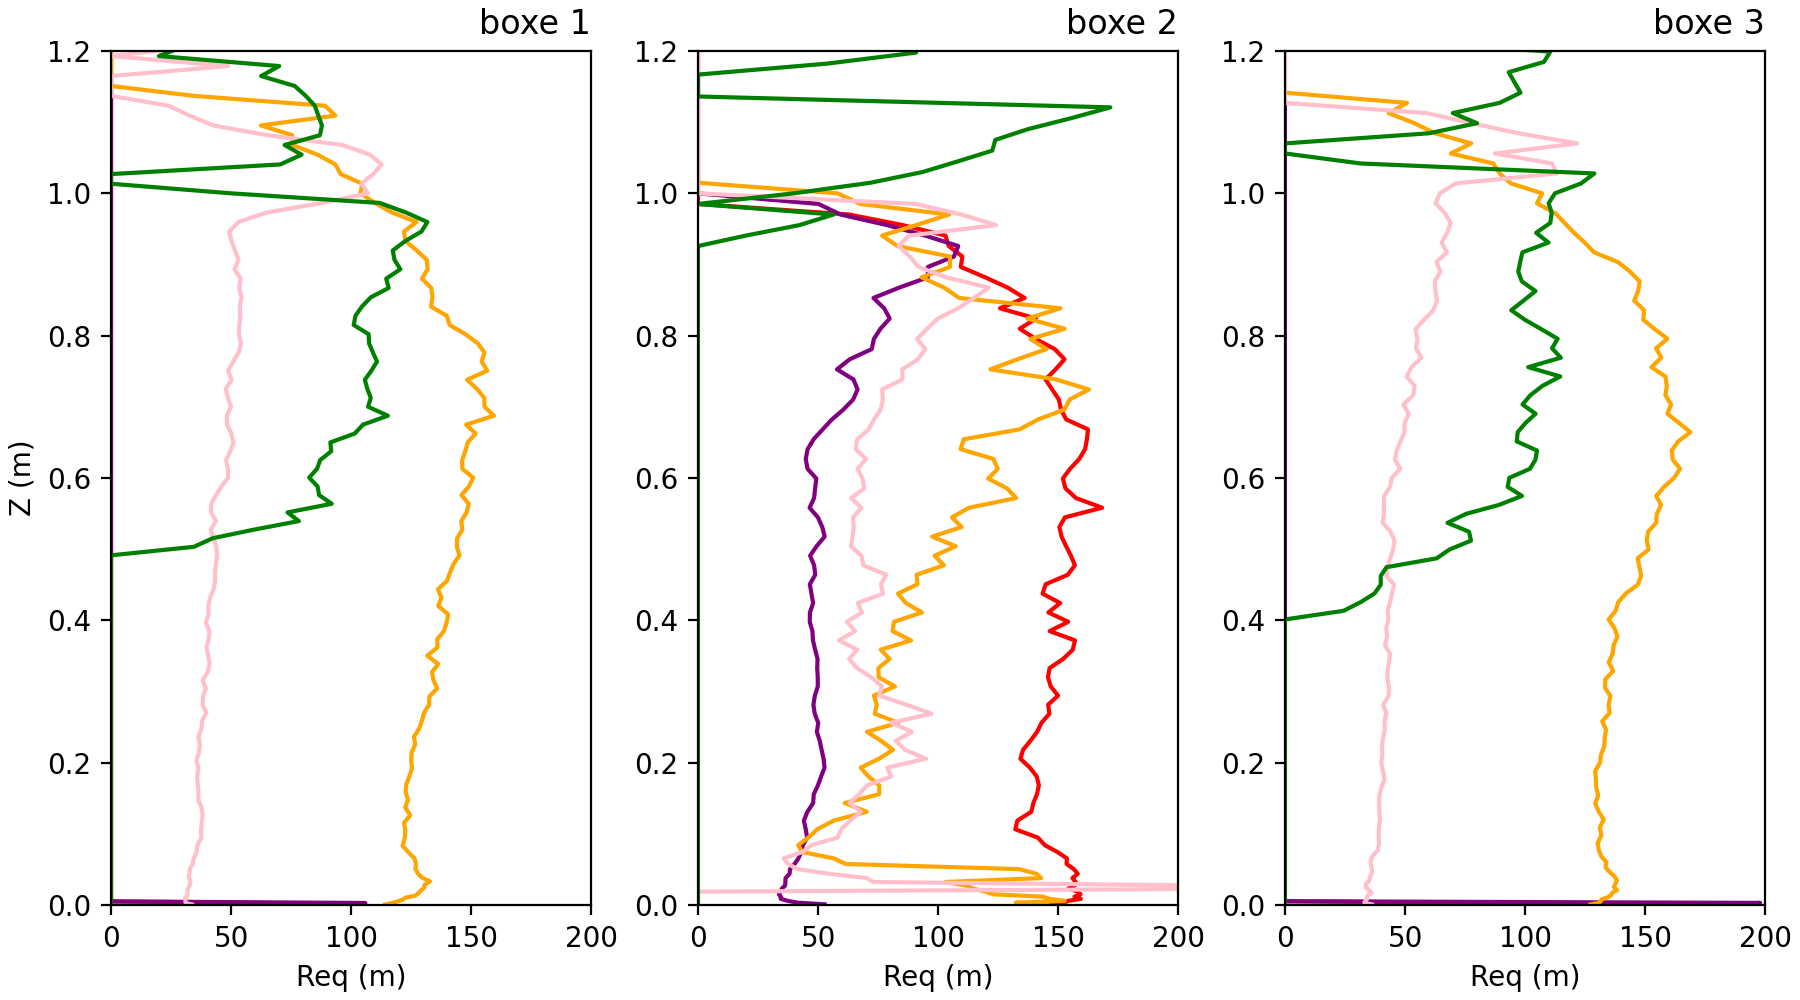
\includegraphics[width=0.99\textwidth]{Requivalent_avg_atZ_allobjects_allLESboxes.png}
    				\caption{Equivalent radius for each object in the LES, averaged over the XY plan for each boxe, at all altitude. Object color is: red for updraft 1, purple for subsiding shell 1, orange for updraft 2, pink for subsiding shell 2 and green for downdrafts.}
    				\label{mean_req}
			    \end{figure} 
            
            \subsection{Linking surface roughness to vertical structure}
            \label{subsection_Link_surface_to_vertical}
            % image on warm part: SAR vs wind surface for different environmental conditions vs uw (or wthtv) decomposition
            % same on cold

            % Un mot sur l'évolution de u* dans la direction along wind ?
            For the length scale identified in the previous section, how can we infer the structure of the ABL from the surface field with the use of coherent structure ? Let's try to give the atmosphere structure (i.e. flux decomposition) above the SAR vignettes. 

            \begin{figure}[h!]
                \centering
                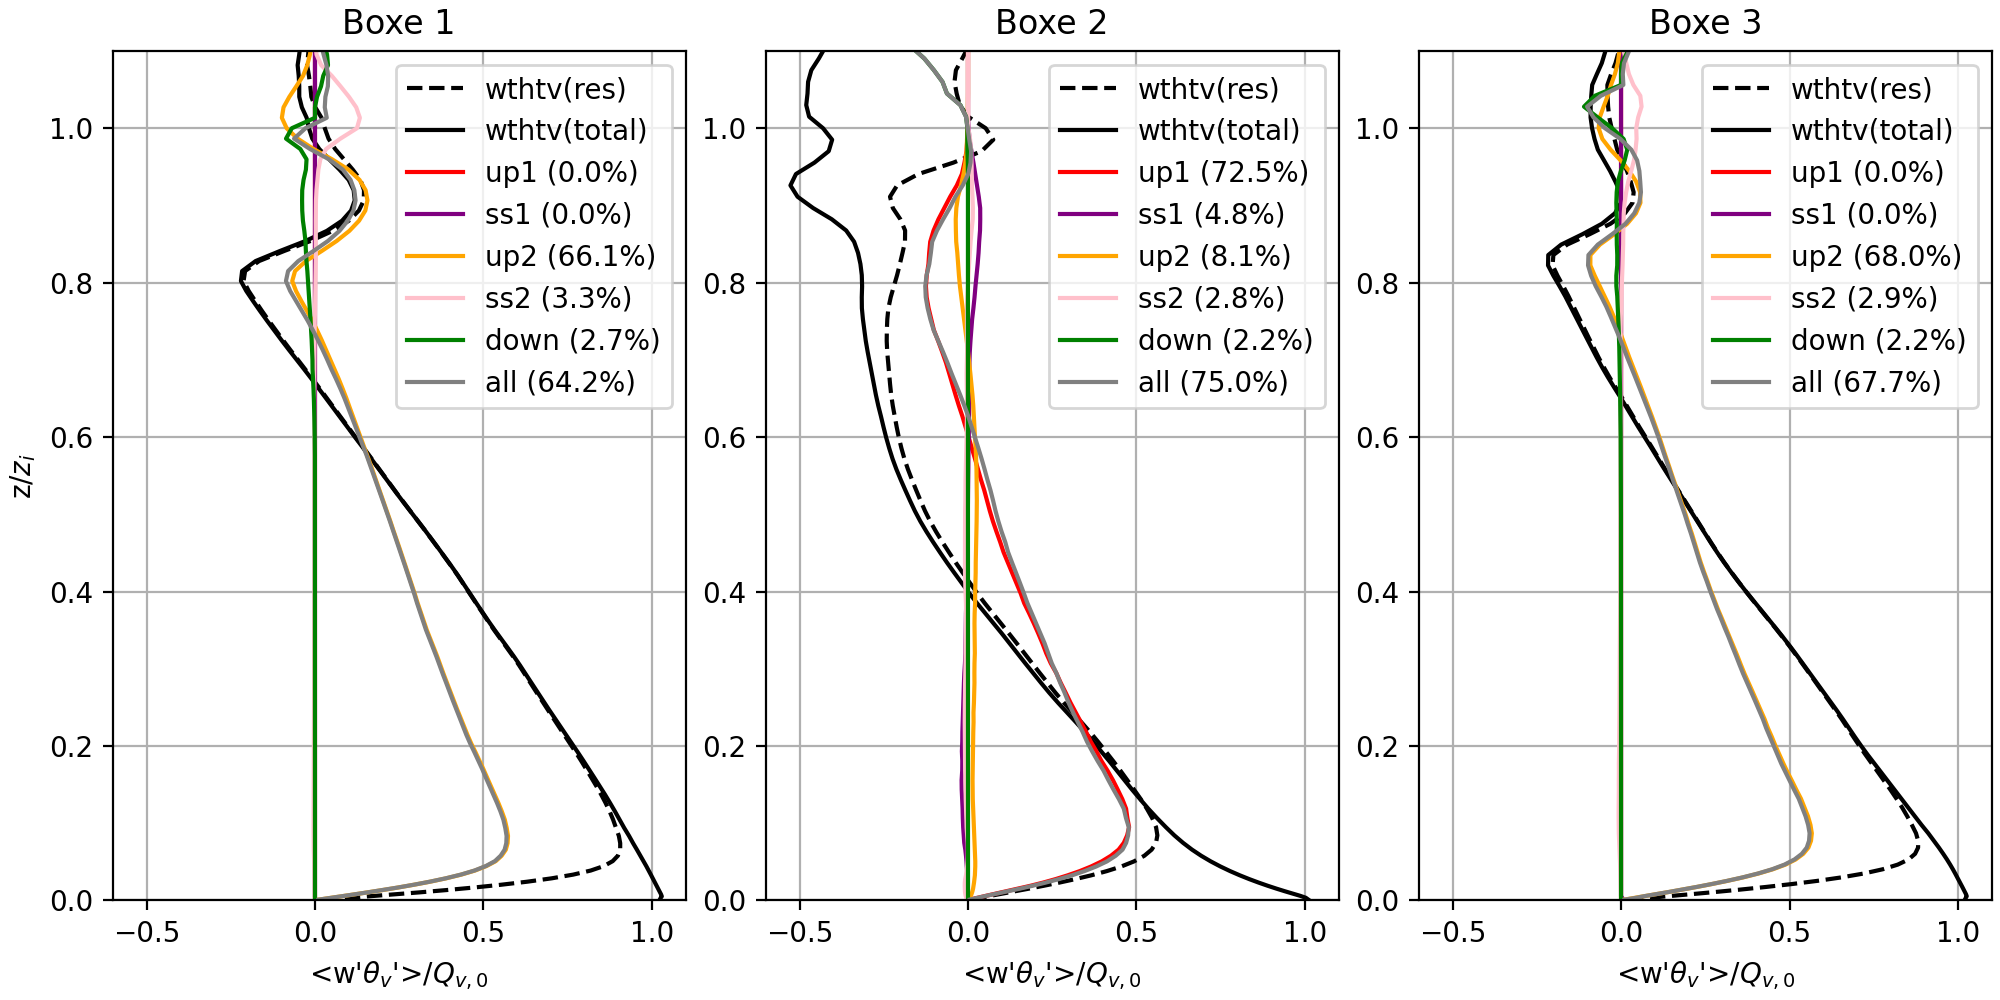
\includegraphics[width=0.99\textwidth]{wthtv_split.png}
                \caption{LES buoyancy flux profile, for each boxes. The flux is decomposed into contributions from coherent structures. Tracer 1: `up' is updrafts and `ss' is subsiding shells. Tracer 2:  `up2' is updrafts and `ss2' is subsiding shells. Tracer 3: `down' is downdrafts. Grey solid line is the contribution from all structure. The percentage in the legend is the vertically integrated contribution.}
                \label{wthtv_CS}
            \end{figure} 
                
            
		\section{Discussion}
		\label{section_discussion}
			
		
		\section{Conclusion}
        \label{section_conclusion}
         


		
		
		\appendix		
			
			
				
				%%%%%%%%%%%%%%%%%%%%%%%%%%%%%%%%%%%%%%%%%%%%%%%
				%
				% DATA SECTION and ACKNOWLEDGMENTS
				%
				%%%%%%%%%%%%%%%%%%%%%%%%%%%%%%%%%%%%%%%%%%%%%%%
				
        \section*{Open Research Section}

        SAR data from Sentinel-1A are made available by the European Copernicus program at WEBSITE. The numerical code used to produce the simulations is MesoNH (version 5.7.0, http://mesonh.aero.obs-mip.fr/mesonh57/Download), namelists and post-process scripts are available on the GitHub repository (https://github.com/HugoJacq/Linking\_SAR\_and\_ABL\_structure).
    
        % This section MUST contain a statement that describes where the data supporting the conclusions can be obtained. Data cannot be listed as ''Available from authors'' or stored solely in supporting information. Citations to archived data should be included in your reference list. Wiley will publish it as a separate section on the paper’s page. Examples and complete information are here:
        %https://www.agu.org/Publish with AGU/Publish/Author Resources/Data for Authors

        % TODO : formater le repo github
        % TODO : envoyer données sur zenodo après retest des namlists
        % voir section 6 pour un exemple https://data.agu.org/resources/agu-data-software-sharing-guidance#guidelines
        % Voir aussi : https://www.agu.org/publish-with-agu/publish/author-resources/data-and-software-for-authors


        \acknowledgments
         
				
			
        %%%%%%%%%%%%%%%%%%%%%%%%%%%%%%%%%%%%%%%%%%%%%%%
        % REFERENCES and BIBLIOGRAPHY
        %
        % \bibliography{<name of your .bib file>} don't specify the file extension
        % don't specify bibliographystyle
        %
        %%%%%%%%%%%%%%%%%%%%%%%%%%%%%%%%%%%%%%%%%%%%%%%
        
        \bibliography{Paper_Agulhas_LES}
        
        \newpage
             		
			
   
			\end{document}
			
			
			
			%More Information and Advice:
			
			%%%%%%%%%%%%%%%%%%%%%%%%%%%%%%%%%%%%%%%%%%%%%%%
			%
			%  SECTION HEADS
			%
			%%%%%%%%%%%%%%%%%%%%%%%%%%%%%%%%%%%%%%%%%%%%%%%
			
			% Capitalize the first letter of each word (except for
			% prepositions, conjunctions, and articles that are
			% three or fewer letters).
			
			% AGU follows standard outline style; therefore, there cannot be a section 1 without
			% a section 2, or a section 2.3.1 without a section 2.3.2.
			% Please make sure your section numbers are balanced.
			% ---------------
			% Level 1 head
			%
			% Use the \section{} command to identify level 1 heads;
			% type the appropriate head wording between the curly
			% brackets, as shown below.
			%
			%An example:
			%\section{Level 1 Head: Introduction}
			%
			% ---------------
			% Level 2 head
			%
			% Use the \subsection{} command to identify level 2 heads.
			%An example:
			%\subsection{Level 2 Head}
			%
			% ---------------
			% Level 3 head
			%
			% Use the \subsubsection{} command to identify level 3 heads
			%An example:
			%\subsubsection{Level 3 Head}
			%
			%---------------
			% Level 4 head
			%
			% Use the \subsubsubsection{} command to identify level 3 heads
			% An example:
			%\subsubsubsection{Level 4 Head} An example.
			%
			%%%%%%%%%%%%%%%%%%%%%%%%%%%%%%%%%%%%%%%%%%%%%%%
			%
			%  IN-TEXT LISTS
			%
			%%%%%%%%%%%%%%%%%%%%%%%%%%%%%%%%%%%%%%%%%%%%%%%
			%
			% Do not use bulleted lists; enumerated lists are okay.
			% \begin{enumerate}
				% \item
				% \item
				% \item
				% \end{enumerate}
			%
			%%%%%%%%%%%%%%%%%%%%%%%%%%%%%%%%%%%%%%%%%%%%%%%
			%
			%  EQUATIONS
			%
			%%%%%%%%%%%%%%%%%%%%%%%%%%%%%%%%%%%%%%%%%%%%%%%
			
			% Single-line equations are centered.
			% Equation arrays will appear left-aligned.
			
			%Math coded inside display math mode \[ ...\]
			% will not be numbered, e.g.,:
			% \[ x^2=y^2 + z^2\]
			%
			% Math coded inside \begin{equation} and \end{equation} will
			% be automatically numbered, e.g.,:
			% \begin{equation}
				% x^2=y^2 + z^2
				% \end{equation}
			
			
			% To create multiline equations, use the
			% \begin{eqnarray} and \end{eqnarray} environment
			% as demonstrated below.
			%\begin{eqnarray}
			%  x_{1} & = & (x - x_{0}) \cos \Theta \nonumber \\
			%        && + (y - y_{0}) \sin \Theta  \nonumber \\
			%  y_{1} & = & -(x - x_{0}) \sin \Theta \nonumber \\
			%        && + (y - y_{0}) \cos \Theta.
			%\end{eqnarray}
			
			%If you don't want an equation number, use the star form:
			%\begin{eqnarray*}...\end{eqnarray*}
			
			% Break each line at a sign of operation
			% (+, -, etc.) if possible, with the sign of operation
			% on the new line.
			
			% Indent second and subsequent lines to align with
			% the first character following the equal sign on the
			% first line.
			
			% Use an \hspace{} command to insert horizontal space
			% into your equation if necessary. Place an appropriate
			% unit of measure between the curly braces, e.g.
			% \hspace{1in}; you may have to experiment to achieve
			% the correct amount of space.
			
			
			%%%%%%%%%%%%%%%%%%%%%%%%%%%%%%%%%%%%%%%%%%%%%%%
			%
			%  EQUATION NUMBERING: COUNTER
			%
			%%%%%%%%%%%%%%%%%%%%%%%%%%%%%%%%%%%%%%%%%%%%%%%
			
			% You may change equation numbering by resetting
			% the equation counter or by explicitly numbering
			% an equation.
			
			% To explicitly number an equation, type \eqnum{}
			% (with the desired number between the brackets)
			% after the \begin{equation} or \begin{eqnarray}
					% command.  The \eqnum{} command will affect only
					% the equation it appears with; LaTeX will number
					% any equations appearing later in the manuscript
					% according to the equation counter.
					%
					
					% If you have a multiline equation that needs only
					% one equation number, use a \nonumber command in
					% front of the double backslashes (\\) as shown in
					% the multiline equation above.
					
					% If you are using line numbers, remember to surround
					% equations with \begin{linenomath*}...\end{linenomath*}
					
					%  To add line numbers to lines in equations:
					%  \begin{linenomath*}
						%  \begin{equation}
							%  \end{equation}
						%  \end{linenomath*}
					
					
					
